\documentclass[a4paper]{article}

\usepackage{hyperref}
\usepackage{amsmath}
\usepackage{tikz}
\usetikzlibrary{automata, positioning, arrows}

\usepackage{graphicx}
\graphicspath{ {./images/static/} }

\tikzset{
->, % makes the edges directed
>=stealth, % makes the arrow heads bold
node distance=3cm, % specifies the minimum distance between two nodes. Change if necessary.
every state/.style={thick, fill=gray!10}, % sets the properties for each ’state’ node
initial text=$ $, % sets the text that appears on the start arrow
}

\begin{document}

\title{Backwards Compatible Automata}
\author{José Duarte}
\date{\today}
\maketitle

\section*{Theory-ish}

We will start by defining one of the simplest state machines — a light bulb.
Using the classical model, the light bulb automata can be defined as follows:

\begin{equation}
    (\Sigma, S, s_0, \delta, F) = (\{click\}, \{\text{Off}, \text{On}\}, \text{Off},S \times \Sigma \rightarrow S, \text{Off})
    \label{eq:fsm_long}
\end{equation}

However, for our purposes we do not need to care for the start nor final states,
for the sake of brevity we will remove them from our automata definitions going forward,
as well as the transition function (which is implicitly defined by stating that our state machines must be DFA).
Hence, we can express our light bulb as follows:

\begin{equation}
    (\Sigma, S) = (\{click\}, \{\text{Off}, \text{On}\})
    \label{eq:fsm_short}
\end{equation}

Which we can observe in \autoref{fig:bulb_fsm}.
The bulb has two states — \emph{On} and \emph{Off} — both of which transition on the application of the symbol $\text{click}$.

\begin{figure}[ht]
    \centering
    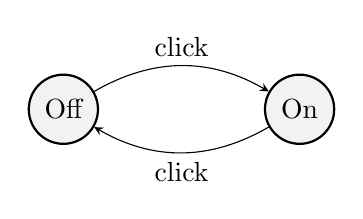
\begin{tikzpicture}
        \node[state] (Off) {Off};
        \node[state, right of=Off] (On) {On};

        \draw (Off) edge[bend left, above] node{click} (On);
        \draw (On) edge[bend left, below] node{click} (Off);
    \end{tikzpicture}
    \caption{Light bulb FSM}
    \label{fig:bulb_fsm}
\end{figure}

\subsection*{Let there be light}

Consider now that we are tasked with changing the state from carrying a boolean to a number,
describing the current light bulb intensity.
% Foreshadowing
Maybe in the future, the manufacturer wants the system to work with potentiometers.
To that end, we change the state machine definition from \autoref{eq:fsm_short}
to the following (\autoref{eq:fsm_intensity} and \autoref{fig:bulb_fsm_intensity}):

\begin{equation}
    (\Sigma, S) = (\{click\}, \{0, 1\})
    \label{eq:fsm_intensity}
\end{equation}

\begin{figure}[ht]
    \centering
    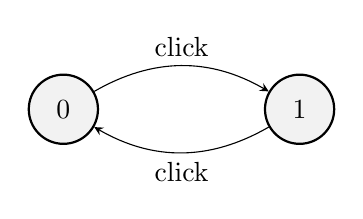
\begin{tikzpicture}
        \node[state] (0) {0};
        \node[state, right of=0] (1) {1};

        \draw (0) edge[bend left, above] node{click} (1);
        \draw (1) edge[bend left, below] node{click} (0);
    \end{tikzpicture}
    \caption{Light bulb FSM with Light intensity}
    \label{fig:bulb_fsm_intensity}
\end{figure}

% I'm dumping the swarm here out of nowhere, this of course, needs an introduction
At first sight, this is not a problem, in code we can just replace the old boolean for an integer,
this would be fine if every node of the swarm could be required to update, but that is not the case.
To cope with said problem, we need to map the old states to the new ones,
using Cambria \cite{Cambria2020} we can convert state information (see \autoref{fig:bulb_fsm_state_cambria}).

\begin{figure}[ht]
    \centering
    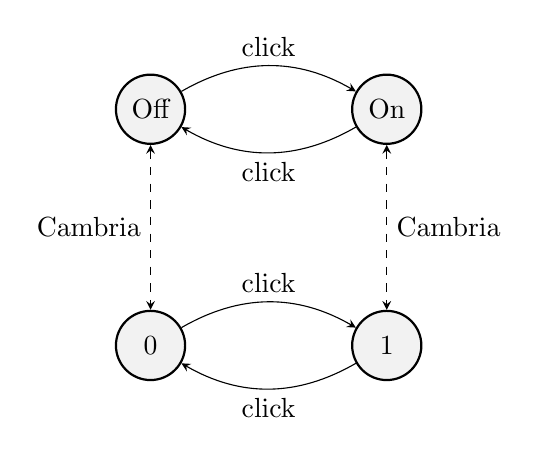
\begin{tikzpicture}
        % Named FSM
        \node[state] (Off) {Off};
        \node[state, right of=Off] (On) {On};

        \draw (Off) edge[bend left, above] node{click} (On);
        \draw (On) edge[bend left, below] node{click} (Off);

        % Intensity FSM
        \node[state, below of=Off] (0) {0};
        \node[state, below of=On] (1) {1};

        \draw (0) edge[bend left, above] node{click} (1);
        \draw (1) edge[bend left, below] node{click} (0);

        \draw (Off) edge[left, <->, dashed] node{Cambria} (0);
        \draw (On) edge[right, <->, dashed] node{Cambria} (1);
    \end{tikzpicture}
    \caption{Light bulb FSM with Cambria state mapping}
    \label{fig:bulb_fsm_state_cambria}
\end{figure}

Along with state conversion, we can extend Cambria to event labels (see \autoref{fig:bulb_fsm_event_cambria}),
which is arguably an even better match since the labels (or payloads for more involved cases)
are what cross the network boundary.

\begin{figure}[ht]
    \centering
    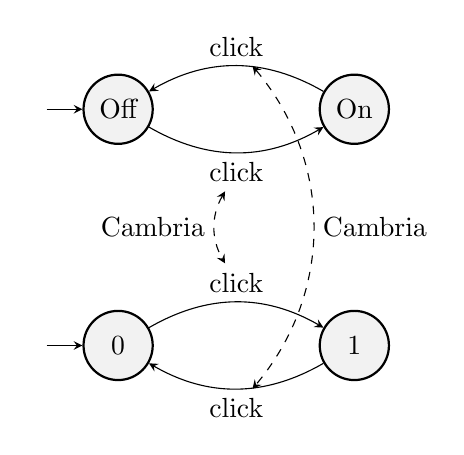
\begin{tikzpicture}
        % Named FSM
        \node[state, initial] (Off) {Off};
        \node[state, right of=Off] (On) {On};

        \draw (On) edge[bend right, above] node (v1-click-off) {click} (Off);
        \draw (Off) edge[bend right, below] node (v1-click-on) {click} (On);

        % Intensity FSM
        \node[state, initial, below of=Off] (0) {0};
        \node[state, below of=On] (1) {1};

        \draw (0) edge[bend left, above] node (v1'-click-on) {click} (1);
        \draw (1) edge[bend left, below] node (v1'-click-off) {click} (0);

        \draw (v1-click-on) edge[bend right, left, <->, dashed] node {Cambria} (v1'-click-on);
        \draw (v1-click-off) edge[bend left=40, right, <->, dashed] node {Cambria} (v1'-click-off);
    \end{tikzpicture}
    \caption{Light bulb FSM with Cambria event mapping}
    \label{fig:bulb_fsm_event_cambria}
\end{figure}

There is still an issue left to address: \emph{How does the old state machine know about new transformations?}
— to which the answer is simple — \emph{It does not know. It cannot know.}

If the old machine were able to get the new transformation,
it would mean that it could get the new state machine as well,
so we need to assume it cannot get the new Cambria transformation.

Thus, we are dealing with an asymmetric scenario where to keep the system running,
the most up-to-date system needs to pick up the slack from the older participants.
To do so, the up-to-date system can either pre-process all information going in and out
(as shown in \autoref{fig:cambria_on_node_translation}) or require that all participants are
at least capable of running arbitrary Cambria transformations and exchange data with
the information of which transformations to apply along with the data
(as shown in \autoref{fig:cambria_payload_with_translation}).

\begin{figure}
    \centering
    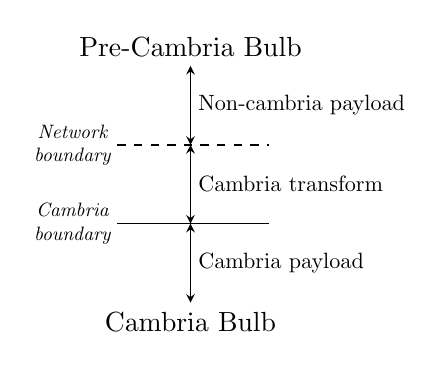
\begin{tikzpicture}
        \node (pre-cambria) at (0, 1.25) {Pre-Cambria Bulb} ;
        \node (cambria) at (0, -2.25) {Cambria Bulb};
        \node[align=center, scale=0.7, font=\itshape] (network) at (-1.5, 0) {Network\\boundary};
        \node[align=center, scale=0.7, font=\itshape] (cambria-b) at (-1.5, -1) {Cambria\\boundary};

        \draw[-, dashed, thick] (network) -- (1, 0);
        \draw[-] (cambria-b) -- (1, -1);

        \draw[<->] (pre-cambria) -- node[right, scale=0.8]{Non-cambria payload} (0, 0);
        \draw[<->] (0, 0) -- node[right, scale=0.8]{Cambria transform} (0, -1);
        \draw[<->] (cambria) -- node[right, scale=0.8]{Cambria payload} (0, -1);
    \end{tikzpicture}
    \caption{Asymmetric interaction between two bulbs, using Cambria to mediate data between them.}
    \label{fig:cambria_on_node_translation}
\end{figure}

\begin{figure}
    \centering
    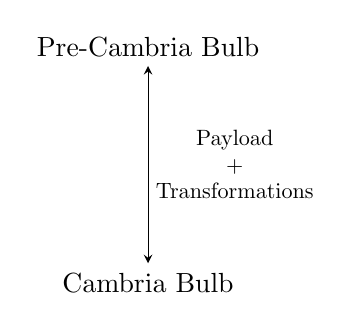
\begin{tikzpicture}
        \node (pre-cambria) {Pre-Cambria Bulb} ;
        \node[below of=pre-cambria] (cambria)  {Cambria Bulb};
        \draw[<->, align=center, right] (pre-cambria) -- node[scale=0.8]{Payload\\$+$\\Transformations} (cambria);
    \end{tikzpicture}
    \caption{Asymmetric interaction between two bulbs, using Cambria to mediate data between them.}
    \label{fig:cambria_payload_with_translation}
\end{figure}


\subsection*{Proper transforms now}

Once again, consider the light bulb using the intensity as states,
imagine that a new change was requested — instead of a toggle, we are now using
a button that can switch intensity from $0$, to $0.5$, to $1$ and back to $0$ (see \autoref{eq:fsm_clicker}).

\begin{equation}
    (\Sigma, S) = (\{click\}, \{0, 0.5, 1\})
    \label{eq:fsm_clicker}
\end{equation}

\begin{figure}[ht]
    \centering
    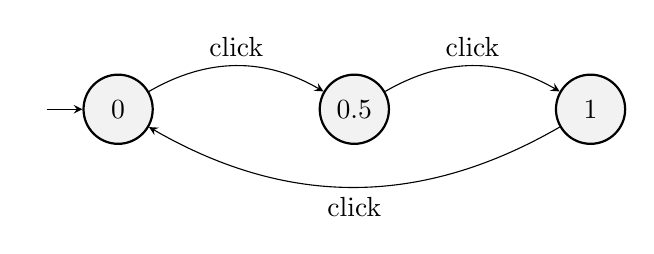
\begin{tikzpicture}
        \node[state, initial] (0) {0};
        \node[state, right of=0] (05) {0.5};
        \node[state, right of=05] (1) {1};

        \draw (0) edge[bend left, above] node{click} (05);
        \draw (05) edge[bend left, above] node{click} (1);
        \draw (1) edge[bend left, below] node{click} (0);
    \end{tikzpicture}
    \caption{Light bulb with support for multiple intensities (as defined in \autoref{eq:fsm_clicker}).}
    \label{fig:bulb_fsm_multi_intensity}
\end{figure}

Usually, we would first design the new state machine (see \autoref{fig:bulb_fsm_multi_intensity})
code it and ship it off as an update to the existing software, replacing the previous state machine.
However, as previously discussed, our system cannot afford the luxury of keeping everyone's version in sync,
so, if we want to support the previous version participants,
we need to keep processing their messages and moving the state machine along.

To support the previous state machine, we start by merging both state machines,
in a more formal way, we can define $merge(M_1, M_2)$
(where $M_1$ and $M_2$ are automata as defined in \autoref{eq:fsm_short}) as:

\begin{equation}
    merge(M_1, M_2) = (M_1.\Sigma \cup M_2.\Sigma, M_1.S \cup M_2.S)
    \label{eq:fsm_merge}
\end{equation}

\begin{figure}[ht]
    \centering
    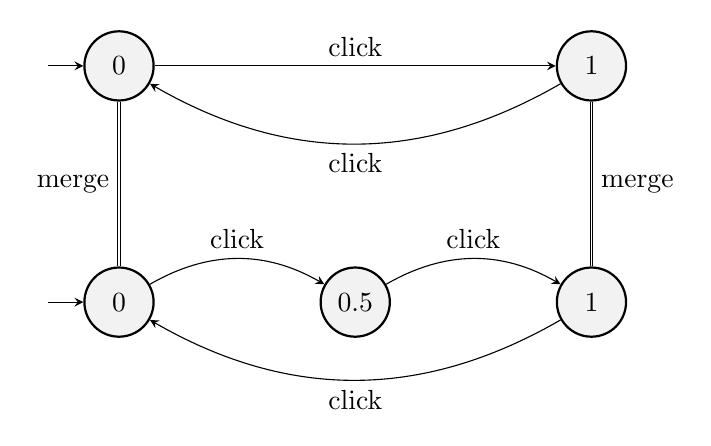
\begin{tikzpicture}
        \node[state, initial] (0) {0};
        \node[state, right of=0] (05) {0.5};
        \node[state, right of=05] (1) {1};

        \draw (0) edge[bend left, above] node{click} (05);
        \draw (05) edge[bend left, above] node{click} (1);
        \draw (1) edge[bend left, below] node{click} (0);

        \node[state, initial, above of=0] (0') {0};
        \node[state, above of=1] (1') {1};

        \draw (0') edge[above] node{click} (1');
        \draw (1') edge[bend left, below] node{click} (0');

        \draw (0) edge[double, -, left] node{merge} (0');
        \draw (1) edge[double, -, right] node{merge} (1');
    \end{tikzpicture}
    \caption{
        Visual approximation of $merge(M_1, M_2)$,
        where $M_1$ is the state machine from \autoref{fig:bulb_fsm} and
        $M_2$ is the state machine from \autoref{fig:bulb_fsm_intensity}.}
    \label{fig:bulb_fsm_merge}
\end{figure}

If we execute $merge$ to the state machines from \autoref{eq:fsm_intensity} and \autoref{eq:fsm_clicker} we get:

\begin{equation}
    \begin{array}{r@{}l}
        merge(M_1, M_2) & {}= (\{click\} \cup \{click\}, \{0, 1\} \cup \{0, 0.5, 1\}) \\
                        & {}= (\{click\}, \{0, 0.5, 1\})
    \end{array}
\end{equation}

Which raises a problem that is not made apparent by the textual representation, but when
displayed visually (see \autoref{fig:bulb_fsm_merge_nfa}) it becomes much more apparent —
notice two outgoing edges from state \emph{0} with the same \emph{click} label; the state machine is now non-deterministic.

% I should probably add this transform as an appendix or something
We can try to make it deterministic, however since we have a single event label and
our states' meaning is different from string matching,
determinization will yield a single state with a single loop labeled \emph{click}
(considering we do not have an accepting state).

The proposed solution is to label edges based on their version, thus removing the "collision" when merging.
If we prefix (or suffix, writers choice) symbols with their version
we are able to preserve the original states and keep the state machine deterministic
as shown in \autoref{fig:bulb_fsm_merge_dfa}.

\begin{equation}
    \begin{array}{r@{}l}
        merge(M_1, M_2) & {}= (\{v1.click\} \cup \{v2.click\}, \{0, 1\} \cup \{0, 0.5, 1\}) \\
                        & {}= (\{v1.click, v2.click\}, \{0, 0.5, 1\})
    \end{array}
    \label{eq:fsm_merge_fixed}
\end{equation}


\begin{figure}[ht]
    \centering
    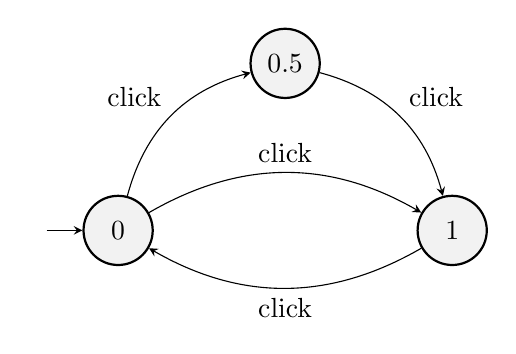
\begin{tikzpicture}
        \node[state, initial] (0) {0};
        \node[state, above right of=0] (05) {0.5};
        \node[state, below right of=05] (1) {1};

        \draw (0) edge[bend left, above left] node{click} (05);
        \draw (0) edge[bend left, above] node{click} (1);
        \draw (05) edge[bend left, above right] node{click} (1);
        \draw (1) edge[bend left, below] node{click} (0);
    \end{tikzpicture}
    \caption{$merge(M_1, M_2)$ results in an NFA (\autoref{eq:fsm_merge}).}
    \label{fig:bulb_fsm_merge_nfa}
\end{figure}

\begin{figure}[ht]
    \centering
    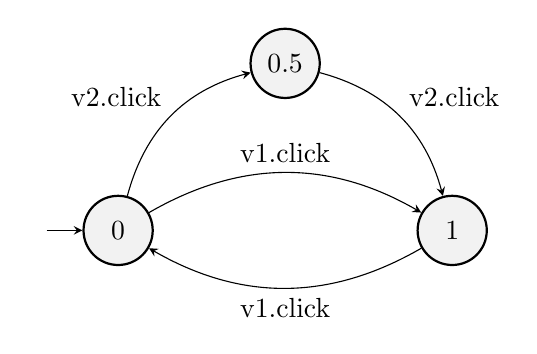
\begin{tikzpicture}
        \node[state, initial] (0) {0};
        \node[state, above right of=0] (05) {0.5};
        \node[state, below right of=05] (1) {1};

        \draw (0) edge[bend left, above left] node{v2.click} (05);
        \draw (0) edge[bend left, above] node{v1.click} (1);
        \draw (05) edge[bend left, above right] node{v2.click} (1);
        \draw (1) edge[bend left, below] node{v1.click} (0);
    \end{tikzpicture}
    \caption{$merge(M_1, M_2)$  with the new labels preserves the DFA (\autoref{eq:fsm_merge_fixed}).}
    \label{fig:bulb_fsm_merge_dfa}
\end{figure}


\begin{figure}[ht]
    \centering
    \includegraphics*[width=5.5cm]{toggle_to_potentiometer}
    \caption{The interface to the bulb may change, requiring new capabilities.}
    \label{fig:to_potentiometer}
\end{figure}

In a regular situation, we would ship this off as an update, however, some systems
cannot guarantee that everyone has updated, thus we are looking to keep backwards compatibility.

To do that, we need to once more, consider the old payloads and states.
We could defer any old payload to the old state machine and create mechanisms to map between both,
however, the new machine did not appear out of nowhere, but rather, it is an evolution
of the original one, so we should treat it as such.

We start by merging the common states and transitions between them.

% Picture here

This way, we have a machine that can handle both cases; almost.

% This doesn't render, write the formula later
If we execute a trace: 0 \-v2\> 0.5 \-v1\> ?
We don't know the final state because it is undefined. To achieve backwards compatibility
we need to address this since the client needs to be able to send actions to the system.

Theorem: When merging state machines, all new states must have outgoing edges for all existing transition labels.

In other words, states from version vn+1 are required to handle all states from vn or less.

States cannot be sinks, meaning that they always need to have at least one outgoing edge (unless they're final states of course).

% Unsure about reachability

Merging is defined by the union of states and transition labels from both the old and new state machine.

If we now want to be able to go back and forth arbitrarily, that is from 0 to 0.5 and back to 0.
Or from 0 to 0.5 to 1 to 0.5, we need to add more events.

To keep backwards compatibility we cannot delete existing parts, but we can create new paths
our previous rule still applies and as such, every new state will be required to handle all previous events.

Unsure: if starting at the initial state, a path is not reachable with older labels,
we can effectively create "feature gates" that stop a user from reaching a weird state.
Feature gates can be done by ignoring previous states (not truly ideal but a valid fallback).


\section*{Runtime-ish}

The state machine must be executed in some type of runtime, which is required to support
a plugin mechanism, be it web assembly modules or OS DLLs.

The way new capabilities are added is additive, in the sense that the state machines are defined
for a single version and merged later (in a pseudo compilation phase that ensures that the current version
is compatible with the previous one and obeys the rules).

When creating a new version, the user shouldn't care to merge automatically, but should care about the
backwards compatible transitions.
The new state machine is described and an automatic checker should validate if both are
compatible, only then is can be "compiled".

Modules should either be additive, meaning that a new module carries only the delta of changes;
or they should be compiled with all previous versions and shipped in a single module.

% Figure this last detail out, it's really important
% The idea would be that the state is a struct carrying data and the new functions handle transitions
% if we have a bunch of free functions, our transitions are something like:
% transition_function(state, event) -> new state
% this way our modules can simply be added cumulatively
% we still need a dynamic dispatch mechanism to pick which function to run
% some kind of switch statement based on the event

\bibliographystyle{plain} % We choose the "plain" reference style
\bibliography{refs} % Entries are in the refs.bib file

\end{document}
